\documentclass[a4paper,10pt]{article}
\usepackage[utf8]{inputenc} % acentos sin codigo
\usepackage{verbatim} % comentarios
\usepackage{graphicx} %imagenes
\usepackage{subfig} %conjuntos de imagenes
\usepackage{listings} %codigo

%opening

\begin{document}
\renewcommand{\listfigurename}{Índice de Figuras}
\renewcommand{\contentsname}{Índice de Contenidos}
\renewcommand{\figurename}{Figura}


%Título
\thispagestyle{empty} 
\title{Alicientes de los videojuegos basados en máquinas de estados}
\author{Leticia López Ortega}
\date{09 de Junio de 2015}
\maketitle
\thispagestyle{empty}
\cleardoublepage

%Agradecimientos
\thispagestyle{empty} 
\begin{flushright}
 \thanks{\emph{Agradecimientos.}} % agradecimientos
\end{flushright}

\cleardoublepage

%Índices
\thispagestyle{empty} 
\tableofcontents
\thispagestyle{empty} 
\cleardoublepage

\addcontentsline{toc}{section}{}
\listoffigures
\thispagestyle{empty} 
\cleardoublepage

%Espacion entre líneas e identación
\setlength{\parindent}{1cm}
\parskip=3mm

%Comienzo de la memoria
\section{Introducción}

\subsection{Introducción}

En el presente proyecto se demuestra la efectividad de máquina de estados orientadas a videojuegos,
mostrando la amplia funcionalidad de esta técnica y sus mejoras en cuanto a refactorización
de código. El juego tiene un modelo de comportamiento en el que pasa por diferentes estados
en los que se determinará funcionalidades propias de cada uno.

\subsection{¿En qu consiste el juego?}

Es un videojuego 2D de naves tipo arcade, en el que se proporciona al jugador la opción de
elegir sus habilidades principales, contando inicialmente con sólo cinco puntos de habilidad.
Tras elegir el jugador se encuentra en un mundo abierto en el que puede viajar con su nave
espacial a diferentes planetas, en dichos planetas habrá un enemigo al que
derrotar, una vez derrotado se recompensa al jugador con un punto de habilidad que podrá
gastar en la habilidad que desee, y seguir así invadiendo planetas, hasta acabar con todos los
enemigos.A parte de la recompensa de un punto de habilidad por haber derrotado a un
enemigo cada 5 enemigos derrotados la nave del jugador se actualizará, haciendo notar al
jugador un avance en el juego y una recompensa por sus habilidades.

\subsection{¿Qué es una máquina de estados?}

Existen varios tipos de máquinas de estados, en este proyecto nos centramos únicamente 
en la máquina de estados finitos, también llamada autómata.\\

Una máquina de estados o autómata, es un modelo de comportamiento, con un conjunto de estados definidos, 
estos estados pueden cambiar mediante entradas y salidas.
Los autómatas se caracterizan por el hecho de tener siempre un estado inicial, cuando reciben una entrada 
pueden cambiar de estado o permanecer en el mismo.
\cleardoublepage

\section{Estado del arte}
\subsection{HTML5}

Es la versión 5 de HTML (HyperText Markup Language). Es un lenguaje basado en etiquetas,
que permite la elaboración de páginas web, definiendo su contenido (imágenes, texto,
videos...) en la versión 5 se incluyen nuevas mejoras.

\subsubsection{Canvas}

Es un elemento de HTML5 que permite generar gráficos estáticos o dinámicos, accediendo a él
mediante código en JavaScript.

\subsection{CSS3}

Es la versión 3 de CSS (Cascading Style Sheets) es un lenguaje que sirve para crear el diseño de
un código HTML, sosteniendo la idea de separar el diseño de una página web de su estructura. 

\subsection{JavaScript}

Es un lenguaje de programación interpretado (quiere decir que no necesita compilación) Es un
lenguaje orientado a objetos, que se basa en prototipos, es débilmente tipado y dinámico.
Normalmente se usa para programar del lado cliente, pero también puede usarse para
programar del lado servidor, gracias a Node.js. Comúnmente se usa para añadir funcionalidad
a las páginas web, dicho código se escribe en un archivo independiente y se enlaza con la
página web.

\subsection{lluviaProject}
Lluvia es un DSL (Domain Specific Language) que se refiere a una especificación de un
lenguaje de programación, en este caso JavaScript, proveyendo al lenguaje de más
funcionalidades de las que posee el lenguaje nativo. Ha sido utilizado para desarrollar la
mayor parte del software de este proyecto.
\cleardoublepage

\subsubsection{Device}
La clase Device es una clase propia de lluviaProject que permite tener un mecanismo de comunicación fluido, 
los Devices son capaces de comunicarse entre ellos mediante eventos, estos eventos son guardados 
en una cola de mensajes. 
Los Device se comunican con el usuario mediante Gates, los cuales son elementos HTML. \\

Los Devices a veces pueden tener un atributo llamdo container, que hace referencia al elemento div de un documento HTML, que se 
muestra cuando se ejecuta el Device.
Los Devices siempre deben tener un atributo llamado self\_events(), que es donde se alamacenan los mensajes que va a recibir.


\subsubsection{States}
Los States son autómatas que proporcionan determinadas funcionalidades en cada instante. Proporcionan gran funcionalidad a 
los Device. Los autómatas siempre deben tener un estado inicial, que será el primero en ejecutarse,
en lluviaProject se define como: running\_up(), después de declarar este State, se pueden declarar más, siempre incluyendo la palabra running.
Al inciar una secuencia de estados el primero siempre de incluir el sufijo \_up.\\

Cuando los States se declaran dentro de un Device el estado running\_up() se ejecutará al mismo tiempo que el Device.
Para cambiar de un state a otro se utiliza la función switch() y entre los parentesis se indicaría el nombre del state al que se desea cambiar.\\

\subsubsection{Gates}
Son puertas de entrada-salida por las que se envían los eventos con los cuales se comunican los
Device, también permite a los Device comunicarse con los objetos HTML, siempre que se le pase el nombre 
del objeto HTML y la función a ejecutar. 
Es necesario que los Gates estén creados dentro de un Device.\\

Para crear un Gate se usa la funcion new\_gate(), entre paréntisis se incluiría el nombre del objeto HTML al que se le 
quiera dar la funcionalidad y se específica que es un Gate. Después se escribe la función que debe tener el Gate y desde que Device se
esta lanzando el evento.

\subsubsection{Boids}
La clase Boid es una inteligencia artificial, en la que cada boid es programado con un comportamiento
independiente del resto de boids, tiene varios comportamientos ya definidos, pero tambien se le pueden agregar 
comportamientos nuevos para funcionalidades más específicas.\\

A los Boids hay que especificarles el canvas en el que se tienen que pintar y el contexto.\\


\cleardoublepage

\section{Arquitectura de la aplicación}
La arquitectura de esta aplicación se ha desarrollado con el patrón Modelo - Vista - Controlador.\\

La aplicación se ha desarrollado principalmente con JavaScript un lenguaje orientado a objetos que 
basa muchas de sus caracterisiticas en la programación dirigida por eventos.\\

La aplicacion está ordenada en clases, las cuales contienen métodos que le agregan funcionalidad.\\

A continuación se muestran el patrón MVC, las clases que contiene la aplicación y los métodos que las clases utilizan.
\cleardoublepage

\subsection{Patrón Modelo - Vista - Controlador}
Es un patron de arquitectura de software utilizado para separar los datos y la lógica del proyecto de la interfaz
de usuario, permitiendo así la separación de conceptos.\\

En este proyecto el controlador sería el Device Game, el modelo son el resto de Devices (PointDealer, Space y Planet) y la vista sería la interfaz de 
usuario desarrollada con HTML5 y CSS3, es decir la aplicación web que vee el usuario.\\

\begin{center}
 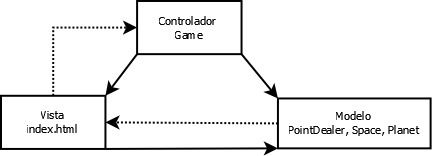
\includegraphics[width=1\textwidth]{./diagrams/diagrama_mvc}
\end{center}

De esta manera Game se comunica con todos los Devices, enviándoles eventos y diciendo cuando se tienen que mostrar. 
Los Devices se comunican con el usuario mediante la interfaz, que sería la aplicación web que se muestra al usuario, y las opciones elegidas por
esté se le mandarían a Game o al Device que se este mostrando, dependiendo del evento que se ejecute cuando el usuario interactua
con la aplicación podría ser el Device mostrado o Game quien recibiera el evento. La respuesta del evento sería notificada al usuario mediante la interfaz.
En caso Game de nuevo se las enviaría al resto de Devices y así sucesivamente, ya que es un patron cíclico.
\cleardoublepage

\subsection{Programación dirigida por eventos}

Es un paradigma de programación, en el que la estructura y la ejecución del 
programa se dirige mediante eventos.
En este tipo de programación se definen los eventos, que manejan el programa y las acciones 
que ocurriran al ejecutarse cada uno de ellos. Al ejecutarse el programa se llevaran a cabo las inicializaciones 
de los elementos que este contenga, y el programa quedará parado hasta que se produzca algún evento,
cuando un evento se ejecuta, se acciona la parte de código definida en el evento, dando lugar
a una respuesta. Esta programación es usada mayormente en interfaces de usuario, ya sean web o de 
escritorio.\\

En el caso de este proyecto, los eventos son inciados por el usuario al pinchar con el
puntero del ratón en alguno de los elementos HTML, o pulsar una tecla del teclado.
En ese momento un evento se ejecuta y realiza una acción que es mostrada al usuario mediante
la interfaz de usaurio de la página web.\\

\emph{Ver diagrama de estados de los eventos, página 28}

\subsection{Clases}

Una clase es un modelo o plantilla diseñado para crear objetos, las clases poseen atributos y
métodos y los objetos los heredan. Cuando un objeto se crea a partir de una clase se llama
instanciación de la clase.\\

\emph{Ver diagramas de clases, página 25 y 26}

\subsubsection{Game}
Es una clase que hereda de la clase Device, este Device es diferente al resto mencionados después, pues es el controlador de la aplicación
y no tiene interfaz, ya que sus tareas no tienen por qué ser visibles al usuario.
La función principal de Game es enviar eventos a otros Devices y recibir las respuestas, para así continuar la ejecución del software, basándose
en el comportamiento de una máquina de estados y en la programación dirigida por eventos, 
recibe una entrada cambia de estado y envía un salida.\\

Por ejemplo: Game envía el evento \textbf{attend\_choosen\_finished()} a PointDealer, diciéndole a PointDealer que cuando el usuario termine
de elegir sus habilidades le mande una respuesta. Cuando Game recibe la respuesta, lanza una alerta diciendole al jugador como ha repartido
sus puntos.

\subsubsection{PointDealer}
Es una clase que hereda de la clase Device, cuya funcionalidad 
es repartir puntos de habilidad al jugador, con un máximo determinado.\\

Las habilidades en las que puede repartir los puntos son \emph{“damage”}, 
\emph{“resistance”} y \emph{“speed”}. Esta clase tiene una interfaz con la que se 
comunica en todo momento el jugador. Esta provista de 2 botones (button\_plus
y button\_minus) con los que el jugador puede aumentar o diminuir los 
puntos de cada habilidad, estos botones son Gates y comunican al Device las acciones realizadas por el jugador, 
si disminuye los puntos se utiliza el método \textbf{get\_back\_from()} y si aumenta los puntos se utiliza el método \textbf{transfer\_to()}.\\

Posee otro botón (button\_play) el cuál tiene la funcionalidad de enviar al 
jugador al siguiente Device, únicamente si el jugador ha gastado todos los 
puntos de habilidad.

\subsubsection{Space}
Es una clase que hereda de la clase Device, 
en Space se crean veinte Gates siendo cada uno de ellos un planeta
diferente al que el jugador podrá viajar, pero no todos ellos se muestran 
en el canvas.\\

Space posee cuatro botones cada uno en un margen del canvas, 
sirviendo al jugador la funcionalidad de desplazarse por el universo en 
busca de diferentes planetas, siendo elección libre para el jugador cual 
escoger. 
\cleardoublepage

\subsubsection{Planet}
Es una clase que hereda de la clase Device, en el que se desarrolla 
la pelea contra el jugador, aquí se crean dos boids (Player y Enemy).
En Planet se crean los boids gracias al método \textbf{initialize()} y es el mundo en el 
que existen.
Planet tiene un método llamado \textbf{attend\_show\_planet()} que pinta una alerta que muestra al jugador el planeta al que esta viajanado.

\subsubsection{Player}
Es una clase que hereda de la clase Boid. Este boid está totalmente 
controlado por el jugador mediante el teclado, no tiene ningún comportamiento 
programado, pero sí algunos de los atributos, como la vida, la posición y
el sprite. Los atributos no programados que podrá escoger el jugador son, 
damage, resistance y speed, se eligen al inicio del juego en el Device 
pointDealer.

\subsubsection{Enemy}
Es una clase que hereda de la clase Boid, creando un array de Boids 
que tienen comportamientos definidos, los cuales son, moverse y atacar.
Cada enemigo es diferente dependiendo del planeta al que viaje el jugador, 
los atributos que cambian son, la vida, el sprite, damage, resistance y speed. El único atributo no variable que posee Enemy es la posición.

\cleardoublepage


\subsection{Métodos}
Un método es un fragmento de código definido dentro de una clase, a la cuál le proporciona una funcionalidad definida en este.
Los objetos creados a partir de dicha clase, tambien podran usar los metodos definidos en ella.
 
\subsubsection{Métodos de PointDealer}
\begin{itemize}
 \item \textbf{get\_back\_from()}: Permite disminuir los puntos de habilidad, 
 de la habilidad en la cual se esté pulsando el (button\_minus).
 \item \textbf{transfer\_to()}: Realiza la tarea opuesta a \textbf{get\_back\_from()}, pues si este quita puntos, 
 \textbf{transfer\_to()} los suma hasta llegar al máximo de puntos permitido, cuando el usuario pulsa el botón (button\_plus).
 \item \textbf{render()}: Cambia las imágenes de la barra de puntos de cada habilidad dependiendo del botón que pulse el jugador. 
 Dando a conocer al usuario los puntos que esta agregando o quitando en cada momentos y en cada habilidad.
 \item \textbf{attend\_show\_skills()}: Permite que Point Dealer se muestre al iniciar el juego.
\end{itemize}


\subsubsection{Métodos de Space}
\begin{itemize}
 \item \textbf{attend\_show\_space()}: Permite que Space se muestre cuando el jugador a pulsado el botón (button\_play)  de Point Dealer.
 \item \textbf{up()}: Proporciona la funcionalidad del botón situado encima del canvas para mover el mapa de los planetas hacia arriba.
 \item \textbf{right()}: Proporciona la funcionalidad del botón situado a la derecha del canvas para mover el mapa de los planetas hacia la derecha.
 \item \textbf{down()}: Proporciona la funcionalidad del botón situado debajo del canvas para mover el mapa de los planetas hacia abajo.
 \item \textbf{left()}: Proporciona la funcionalidad del botón situado a la izquierda del canvas para mover el mapa de los planetas hacia la izquierda.
\end{itemize}


\subsubsection{Métodos de Planet}
\begin{itemize}
 \item \textbf{initialize()}: Inicializa a Player y a Enemy para que se creen en Planet.
 \item \textbf{attend\_show\_planet()}: Hace que el planeta se muestre, con una alerta que indica el número del planeta que es.
 \item \textbf{has\_born()}: Registra que se ha creado un Boid y se envía un mensje a sí mismo.
 \item \textbf{draw()}: Dibuja el canvas en el mundo.
 \item \textbf{new\_boid()}: Crea una nuevo Boid.
 \item \textbf{new\_boid\_of()}: Crea un Boid a partir de una clase de Boids, previamente definida.
 \item \textbf{get\_boids()}: Crea un array con todos los Boids.
 \item \textbf{repaint(ctx)}: Pinta el canvas de negro.
 \item \textbf{resize()}: Permite que el jugador pueda poner el juego en apantalla completa usando el botón (button\_screen).
\end{itemize}


\subsubsection{Métodos de Player}
\begin{itemize}
 \item \textbf{random(max)}: Escoge un número aleatorio para empezar a pintar esrellas en el canvas de Planet.
 \item \textbf{move()}: Hace que se mueva Player, los disparos que lanza y las estrellas del canvas.
 \item \textbf{paint(ctx)}: Pinta a Player, a los disparos, a las estrellas y los FPS.
 \item \textbf{draw()}: Es una función prototípica heredada de Planet, aquí se ejecuta
 el método \textbf{repaint(ctx)}, declarado en Planet, el método \textbf{stars()}, después el método \textbf{move()} y después el método \textbf{paint()} 
 y después se dibuja el Boid Player.
 \item \textbf{stars()}: Pinta en el canvas una lluvia de estrellas creadas a partir de la clase Star.
\end{itemize}


\subsubsection{Métodos de Enemy}
\begin{itemize}
 \item \textbf{move()}: Es donde se define el movimiento de Enemy.
 \item \textbf{draw(ctx)}: Es una función prototípica heredada de Planet que pinta el Boid Enemy.
 \item \textbf{shot()}: Es donde está el código encargado de que Enemy dispare automáticamente cada cierto tiempo.
\end{itemize}
\cleardoublepage

\section{Desarrollo de la aplicación}
\subsection{Entorno utilizado}
Un entorno de desarrollo puede ser una o varia aplicaciones, 
que se compone de un editor de texto, un depurador y un compilador, 
en este caso como el lenguaje utilizado ha sido JavaScript no ha sido 
necesaria la utilización de un compilador.

\subsubsection{SublimeText 3}
Es un editor de texto o editor de código fuente y 
ha sido utilizado para crear todo el código fuente de la aplicación.

\subsubsection{Mozilla Firefox}
Es un navegador web libre y de código abierto. 
Su consola JavaScript ha sido utilizada para comprobar los 
errores en el código fuente y su herramienta de depuración 
incorporada (FireBug), ha sido de gran ayuda a la hora de realizar las tareas de 
testing y debug.

\subsubsection{PhotoShop CS6}
Es un editor de gráficos, con el cual se ha desarrollado 
gran parte de los diseños del videojuego.

\subsubsection{GitHub}
Es un control de versiones on-line, basado en Git, 
desde el cual se descarga lluviaProject y ha sido muy útil 
para ordenar el código y poder portarlo de un ordenador a otro.
\cleardoublepage

\subsection{Librerías utilizadas}

Para completar más el desarrollo gráfico del proyecto se han incluido varias librerias, aportando un diseño
más especifíco.

\subsubsection{SweetAlert}

Es una librería que permite personalizar las alertas de JavaScript, permitiendo cambiar el estilo.
También permite agregar ciertas animaciones ya definidas en la librería.

\subsubsection{Google Fonts}

Es una librería creada por Google, que permite cambiar el tipo de fuente de toda la aplicación web, 
seleccionando una de las fuentes que Google te da para elegir.
\cleardoublepage

\subsection{¿Por qué lluviaProject?}
El presente proyecto se ha querido desarrollar con este lenguaje por que incorporaba funcionalidades necesarias para llevar
a cabo el juego planetado, como por ejemplo los Boids y los States, de esta manera se ha evitado la duplicidad de código y el tener 
que programar toda una inteligencia artificial que ya estaba hecha en lluviaProject.

\subsection{Desarrollo del fundamento del juego: La pelea entre los Boids}
La pelea entre los Boids se desarrolla en el Device Planet ya que es donde se crean los Boids.

Para el funcionamiento de Player se han usado los números de las teclas del teclado definidos en JavaScript:

\begin{verbatim}
var KEY_LEFT  = 37
var KEY_RIGHT = 39
var KEY_SHOT  = 87
\end{verbatim}

Siendo así, que cuando el jugador pulsa una tecla para ir a la derecha, se aumenta el valor de la posición de Player en x según la velocidad
que el jugador seleccionase en el atributo speed de PointDealer, aunque la velocidad siempre sera igual a la velocidad seleccionada + 1,
y cuando pulsa una tecla para ir a la izquierda se disminuye la posición de Player en x de la misma forma que se aumenta.
 
\begin{verbatim}
if (pressing[KEY_RIGHT])
    this.x += this.speed + 1
if (pressing[KEY_LEFT])
    this.x -= this.speed + 1
\end{verbatim}

Los disparos de Player han sido creados gracias a la clase Rectangle, definida dentro de la clase Player, cada vez que el jugador pulsa la tecla w del teclado 
Player dispara un pequeño rectángulo.

\begin{verbatim}
 if (lastPress == KEY_SHOT) {
     this.shots.push(new Rectangle (this.x +38, this.y, 5, 10)) 
     lastPress = null
 }
\end{verbatim}
\cleardoublepage

Los disparos de Player se mueven disminuyendo su coordenada y, ya que el disparo debe de ir hacía la parte de arriba del
canvas, que es donde se encuentra Enemy.

\begin{verbatim}
 for (var i=0, l=this.shots.length; i<l; i++) {
      this.shots[i].y -= 5 //shots speed  
      if (this.shots[i].y < 0) {
         this.shots.splice(i--, 1)
         l--
      }
 }
\end{verbatim}


El movimiento de Enemy se desarrolla gracias a los movimientos definidos de los Boids, habiendo hecho algunos cambios, 
para que solo se pueda desplazar en x.

Los disparos de Enemy no estan terminados.
\cleardoublepage

\subsubsection{Control de colisiones}

Dando por valido que las posiciones de Player y Enemy son:

\begin{center}
 \begin{tabular}{cc}
 \hline
  Player & Enemy\\
  \hline
  \verb| Player.x = 450                   | & \verb|Enemy.x = 460                  |\\
  \verb| Player.y = 460                   | & \verb|Enemy.y = 50                   |\\
  \verb| Player.width = 90                | & \verb|Enemy.width = 120              |\\
  \verb| Player.height = 107              | & \verb|Enmey.height = 90              |\\
  \verb| Player.shots.x = Player.x +38    | & \verb|Enemy.shots.x = Enemy.x +60    |\\
  \verb| Player.shots.y = Player.y        | & \verb|Enemy.shots.y = 120            |\\
  \verb| Player.shots.width = 5           | & \verb|Enemy.shots.width = 5          |\\
  \verb| Player.shots.height = 10         | & \verb|Enemy.shots.height = 5         |\\
 \hline
 \end{tabular}
\end{center}

El algoritmo del control de colisiones entre los disparos de Player y Enemy sería:

\begin{verbatim}
 this.shots.x < enemy.x + enemy.width &&
 this.shots.x + this.shots.width > enemy.x &&
 this.shots.y == enemy.y + enemy.height &&
 this.shots.y + this.shots.height > enemy.y
\end{verbatim}

Como el disparo se mueve en la posición y en algún momento debe ser igual a 50 y chocar contra Enemy.
Sabemos que el algoritmo funciona, probandolo con pseudoćodigo, 
cambiando las variables por el número de la posición asociada:

\begin{verbatim}
 460 < 460 + 50           == true
 460 + 5 > 460            == true
 this.shots.y == 50 + 90  == true
 this.shots.y + 10 > 50   == true
\end{verbatim}
\cleardoublepage


El algoritmo del control de colisones entre los disparos de Enemy y Player sería:

\begin{verbatim}
 this.shots.x < player.x + player.width &&
 this.shots.x + this.shots.width > player.x &&
 this.shots.y == player.y + player.height &&
 this.shots.y + this.shots.height > player.y
\end{verbatim}

Demostramos que el algoritmo funciona mediante pseudocódigo, como en el caso anterior:

\begin{verbatim}
 520 < 460 + 90             == true
 520 + 120 > 450            == true
 this.shots.y == 460 + 107  == true
 this.shots.y + 90 > 460    == true
\end{verbatim}
\cleardoublepage









\section{Diseño}

\subsection{Diseño de interfaz}

La interfaz está diseñada con HTML y CSS siendo esta una interfaz 
sencilla e intuitiva para el jugador.
La primera pantalla se compone de tres barras y tres botones, de 
los cuales la funcionalidad está hecha con JavaScript.
La siguiente pantalla se denominaría como el entorno abierto y 
de libre elección del videojuego, que consiste en una simulación del 
espacio exterior con diversos planetas a los que el jugador puede viajar.

\emph{Ver figuras 1, 2, 3}

\subsection{Diseño de mundo}

Es un diseño de mundo abierto, lo cual quiere decir que el 
juego ofrece al jugador la posibilidad de moverse libremente por 
este y de elegir a donde ir.

\subsection{Diseño de Enemy y Player}

Estos diseños están basados en naves espaciales, pintadas en 2D.

\emph{Ver figuras de 4 a 23}

\subsection{Diseño de nivel}

Es el diseño de escenario o misiones del videojuego, 
lo cual se basa no sólo en el aspecto gráfico sino también 
en la dificultad. Se dice que un juego tiene un buen diseño de nivel 
cuando el jugador nota que el juego avanza y la dificultad cada vez es 
más elevada.\\

En el presente proyecto el aspecto gráfico no se ha desarrollado mucho, 
queriendo darle un aspecto simple y minimalista, sin embargo el desarrollo 
del diseño de nivel en cuanto al aumento de dificultad en cada etapa 
del juego ha sido programado meticulosamente.

\subsubsection{Objetivo y recompensa}

El objetivo del juego es destruir a todos los alienígenas invasores 
de los planetas.
La recompensa es proporcionada al jugador cada vez que este
consigue derrotar a un enemigo, dandole un punto de habilidad 
más para aumentar sus estadísticas y haciéndole posible la victoria 
en la siguiente batalla.

\subsubsection{Dificultad}

El orden de dificultad es el orden numérico de los planetas, 
siendo el planeta 1 el que posee al enemigo más débil y 
el planeta 20 el que posee el enemigo más poderoso.
Al ser un mundo abierto y el jugador no tener consciencia 
sobre el orden de los planetas, hace que la dificultad del 
juego aumente y posiblemente también la curiosidad de saber que 
pasará en el siguiente planeta al que viaje.
\cleardoublepage

\section{Conclusiones}

El objetivo de este proyecto ha sido crear una pequeña muestra de lo que se puede hacer usando 
las máquinas de estados para desarrollar videojuegos.

Las conclusiones obtenidas han sido:

\begin{itemize}
 \item La eficacia de las máquinas de estados para videojuegos, 
 es muy potente y recomendable, aun siendo más dificultosa que un método
 basado en condiciones, se consigue optimizar el código y el tiempo dedicado.
 \item La clase pointDealer puede usarse para muchas más 
 aplicaciones orientadas a videojuegos, ya que es un repartidor, 
 podría distribuir no sólo puntos, sino comida, oro, etc.
 \item El uso de la clase boids en la programación de la 
 inteligencia artificial de los enemigos 
 en videojuegos evita la duplicidad de código.
 \item El desarrollo de autómatas requiere de una programación delicada 
 y el uso de constantes pruebas para comprobar errores.
\end{itemize}

\subsection {Optimizaciones del proyecto}

Este proyecto podría mejorarse, de manera fácil y sencilla, algunas de las mejoras
que se le podría hacer son:

\begin{itemize}
 \item Implementar un nuevo modo de juego, en el que puedan jugar dos jugadores, en un 1 vs 1, haciendo uso de Node.js.
 \item Mejorar el diseño gráfico haciéndolo más apetecible para el público.
 \item Implementar sonidos y músicas dotando al videojuego de realismo.
 \item Crear un apartado de personalización, para que el jugador pueda 
 customizar su avatar como desee.
\end{itemize}

\subsubsection {Posibles aplicaciones}
Podrían usarse algunas de las clases para la creación 
de nuevos videojuegos, por ejemplo Player, Enemy o PointDealer.
\cleardoublepage

\section{Bibliografía}
La información obtenida para el desarrollo de este proyecto ha sido:
\begin{itemize}
 \item lluviaProject Wiki
 \item “Proyecto de Simulación Comportamental en Entornos con Tasas de Estrés Variable”. 
 José Moreno Casero e Iván Bravo del Valle.
 \item “Estudio del comportamiento del ganado en sistemas distribuidos con caracteres autónomos“.
 María Losada, Estefanía Valenzuela y Laura Zorrilla.
\end{itemize}

\cleardoublepage



\appendix
\section{Diagramas}
\subsection{Diagramas de clases}
\subsubsection{Diagrama de clases de Device}
\begin{center}
 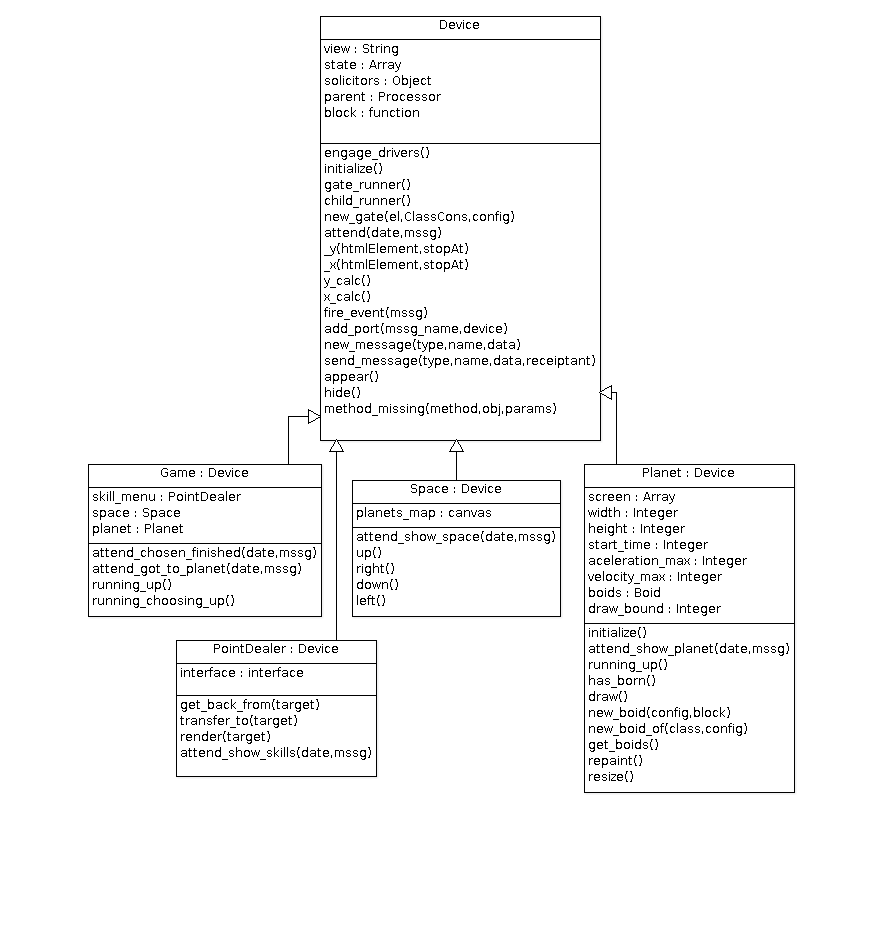
\includegraphics[width=1.3\textwidth]{./diagrams/clases_device}
\end{center}

\subsubsection{Diagrama de clases de Boids}
\begin{center}
 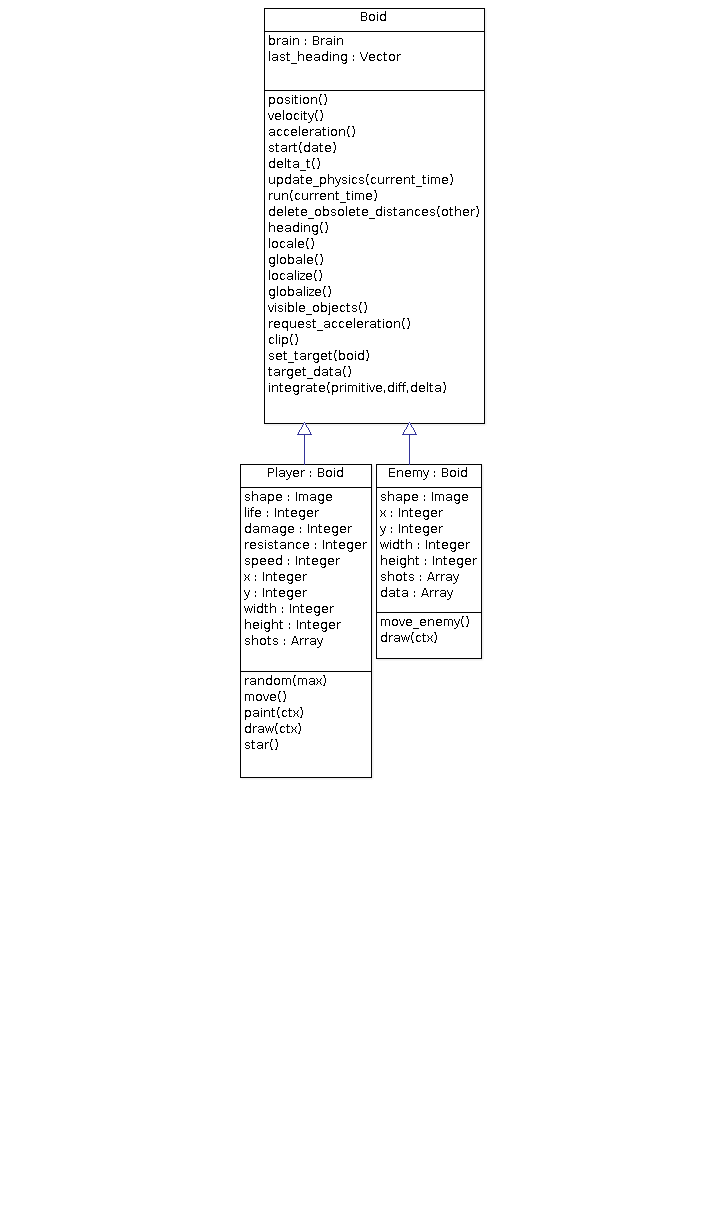
\includegraphics[width=1.3\textwidth]{./diagrams/clases_boids}
\end{center}
\cleardoublepage

\subsection{Diagrama de estados del juego}
\begin{center}
 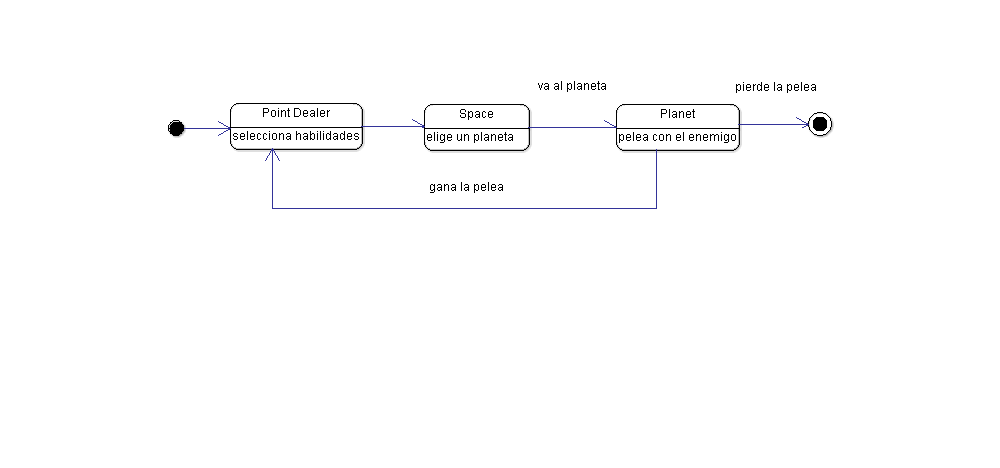
\includegraphics[width=1.2\textwidth]{./diagrams/estados}
\end{center}

\subsection{Diagrama de estados de los eventos}
\begin{center}
 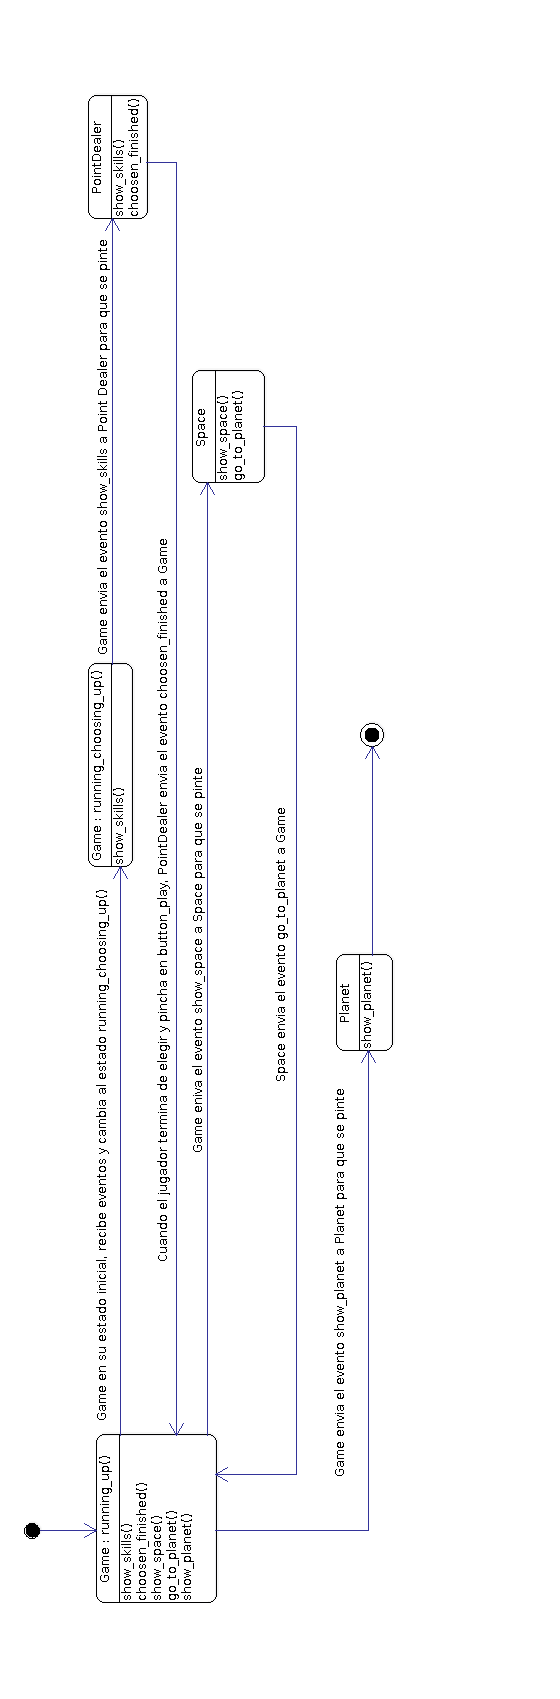
\includegraphics[width=0.5\textwidth]{./diagrams/diagrama_eventos}
\end{center}
\cleardoublepage


%Devices

\begin{figure}[htb]
\centering
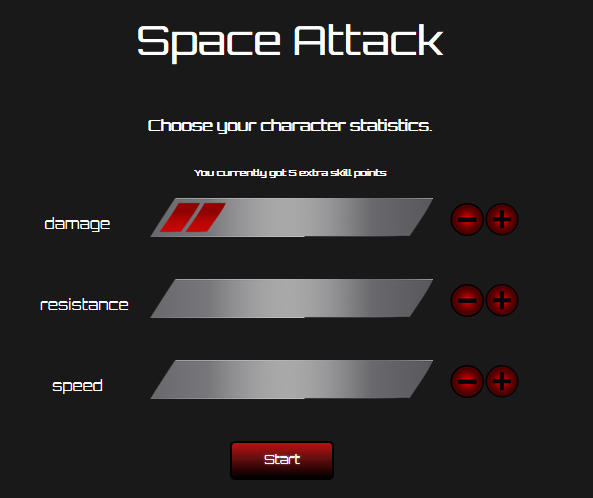
\includegraphics[width=1\textwidth]{point_dealer}
\caption{Device PointDealer}
\label{fig:pointDealer}
\end{figure}

\begin{figure}[htb]
\centering
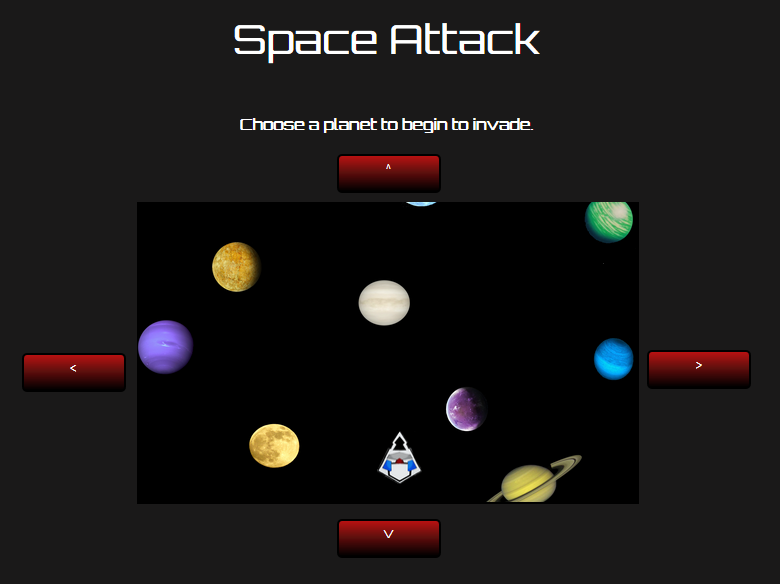
\includegraphics[width=1\textwidth]{space}
\caption{Device Space}
\label{fig:space}
\end{figure}

\begin{figure}[htb]
\centering
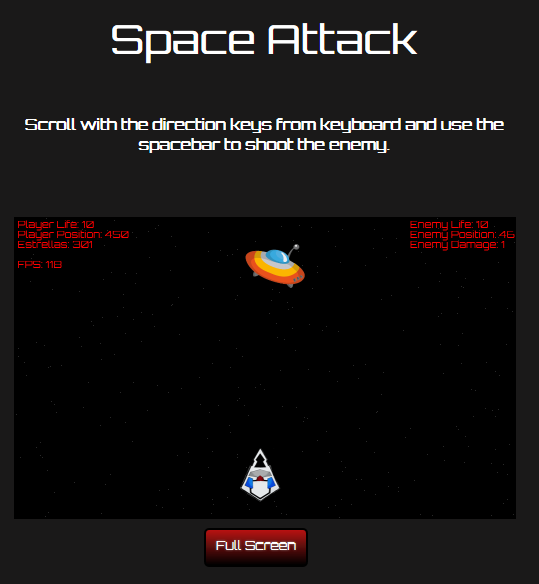
\includegraphics[width=1\textwidth]{planet}
\caption{Device Planet}
\label{fig:planet}
\end{figure}

\cleardoublepage

%Boids
\begin{figure}[htbl!]

%planetas amarillos
\begin{minipage}[b]{0.5\linewidth} %Una minipágina que cubre la mitad de la página
\centering
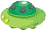
\includegraphics[width=30mm]{./ships/ship0}
\caption{Nave enemiga 1 del planeta 1} \label{figura1}
\end{minipage}
\hspace{0.5cm} % Espacio entre figuras
\begin{minipage}[b]{0.5\linewidth}
\centering

\includegraphics[width=30mm]{./ships/ship1}
\caption{Nave enemiga 2 del planeta 2} \label{figura2}
\end{minipage}

\end{figure}


\begin{figure}[htbl!]

\begin{minipage}[b]{0.5\linewidth}
\centering

\includegraphics[width=30mm]{./ships/ship2}
\caption{Nave enemiga 3 del planeta 3} \label{figura3}
\end{minipage}
\hspace{0.5cm} % Espacio entre figuras
\begin{minipage}[b]{0.5\linewidth}
\centering
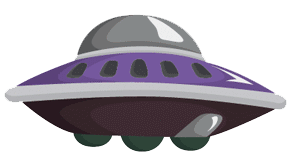
\includegraphics[width=30mm]{./ships/ship3}
\caption{Nave enemiga 4 del planeta 4} \label{figura4}
\end{minipage}

\end{figure}

\begin{figure}[htbl!]

\begin{minipage}[b]{0.5\linewidth}
\centering

\includegraphics[width=30mm]{./ships/boss0}
\caption{Nave enemiga 5 del planeta 5} \label{figura5}
\end{minipage}
%Planetas naranjas y rojos
\hspace{0.5cm}
\begin{minipage}[b]{0.5\linewidth}
\centering

\includegraphics[width=30mm]{./ships/ship4}
\caption{Nave enemiga 6 del planeta 6} \label{figura6}
\end{minipage}

\end{figure}

\begin{figure}

\begin{minipage}[b]{0.5\linewidth}
\centering
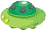
\includegraphics[width=30mm]{./ships/ship5}
\caption{Nave enemiga 7 del planeta 7} \label{figura7}
\end{minipage}
\hspace{0.5cm}
\begin{minipage}[b]{0.5\linewidth}
\centering

\includegraphics[width=30mm]{./ships/ship6}
\caption{Nave enemiga 8 del planeta 8} \label{figura8}
\end{minipage}

\end{figure}


\begin{figure}

\begin{minipage}[b]{0.5\linewidth}
\centering

\includegraphics[width=30mm]{./ships/ship7}
\caption{Nave enemiga 8 del planeta 8} \label{figura8}
\end{minipage}
\hspace{0.5cm}
\begin{minipage}[b]{0.5\linewidth}
\centering

\includegraphics[width=30mm]{./ships/boss1}
\caption{Nave enemiga 9 del planeta 9} \label{figura9}
\end{minipage}

\end{figure}

%planetas morados
\begin{figure}

\begin{minipage}[b]{0.5\linewidth}
\centering
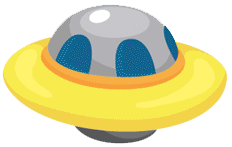
\includegraphics[width=30mm]{./ships/ship8}
\caption{Nave enemiga 10 del planeta 10} \label{figura10}
\end{minipage}
\hspace{0.5cm}
\begin{minipage}[b]{0.5\linewidth}
\centering

\includegraphics[width=30mm]{./ships/ship9}
\caption{Nave enemiga 11 del planeta 11} \label{figura11}
\end{minipage}

\end{figure}


\begin{figure}

\begin{minipage}[b]{0.5\linewidth}
\centering

\includegraphics[width=30mm]{./ships/ship10}
\caption{Nave enemiga 12 del planeta 12} \label{figura12}
\end{minipage}
\hspace{0.5cm}
\begin{minipage}[b]{0.5\linewidth}
\centering
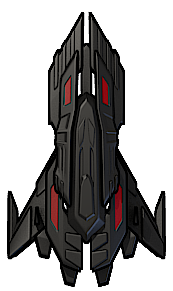
\includegraphics[width=30mm]{./ships/boss2}
\caption{Nave enemiga 13 del planeta 13} \label{figura13}
\end{minipage}

\end{figure}

%planetas azules y verdes
\begin{figure}

\begin{minipage}[b]{0.5\linewidth}
\centering

\includegraphics[width=30mm]{./ships/ship11}
\caption{Nave enemiga 14 del planeta 14} \label{figura14}
\end{minipage}
\hspace{0.5cm}
\begin{minipage}[b]{0.5\linewidth}
\centering
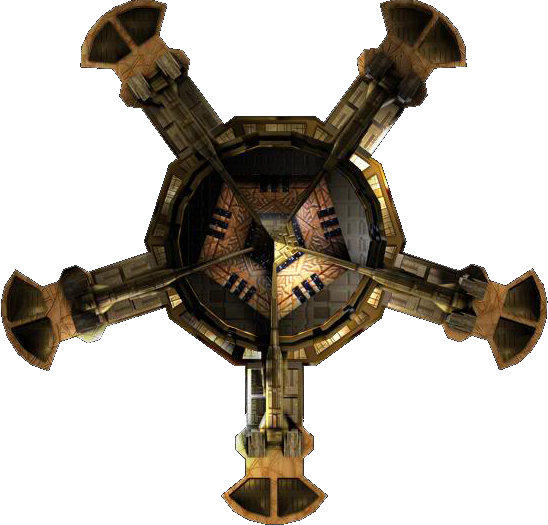
\includegraphics[width=30mm]{./ships/ship12}
\caption{Nave enemiga 15 del planeta 15} \label{figura15}
\end{minipage}

\end{figure}

\begin{figure}

\begin{minipage}[b]{0.5\linewidth}
\centering
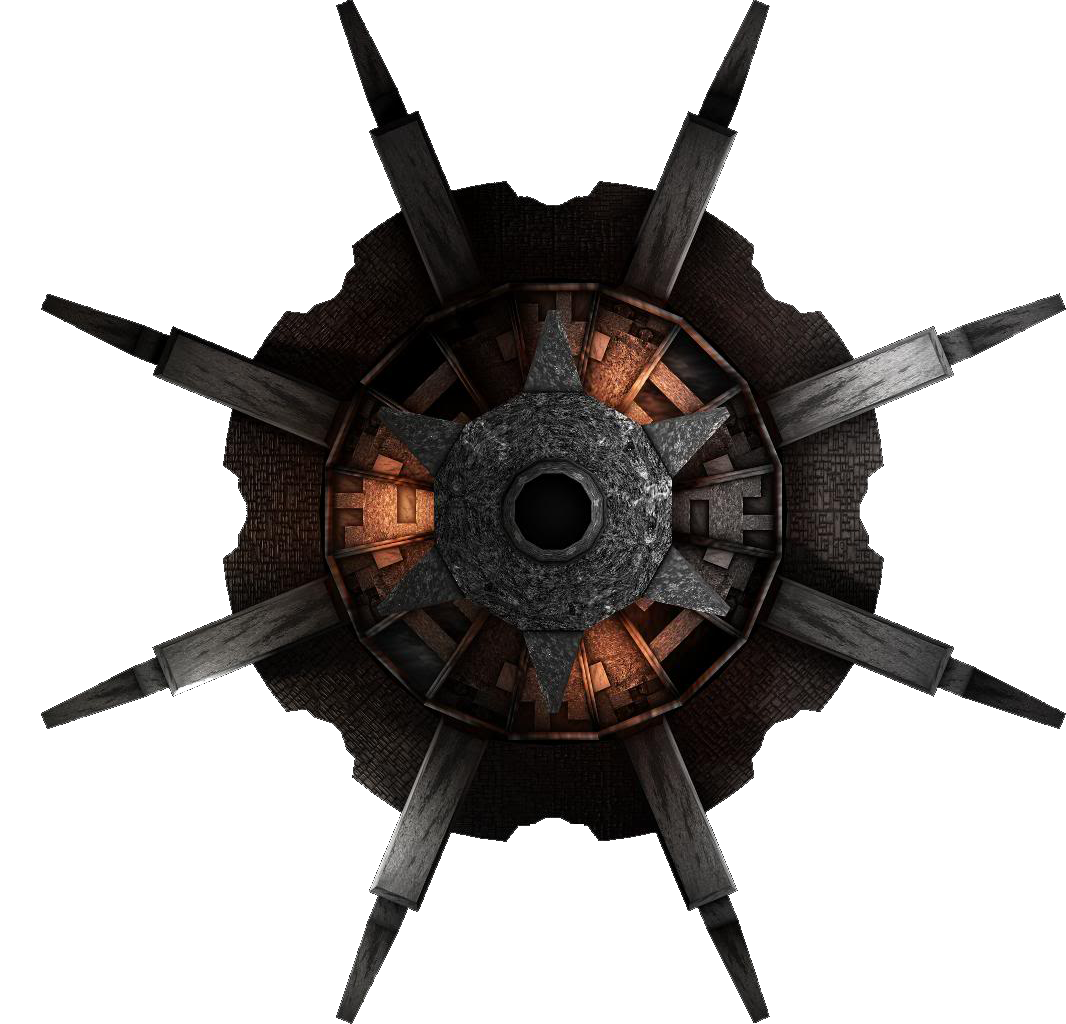
\includegraphics[width=30mm]{./ships/ship13}
\caption{Nave enemiga 16 del planeta 16} \label{figura16}
\end{minipage}
\hspace{0.5cm}
\begin{minipage}[b]{0.5\linewidth}
\centering
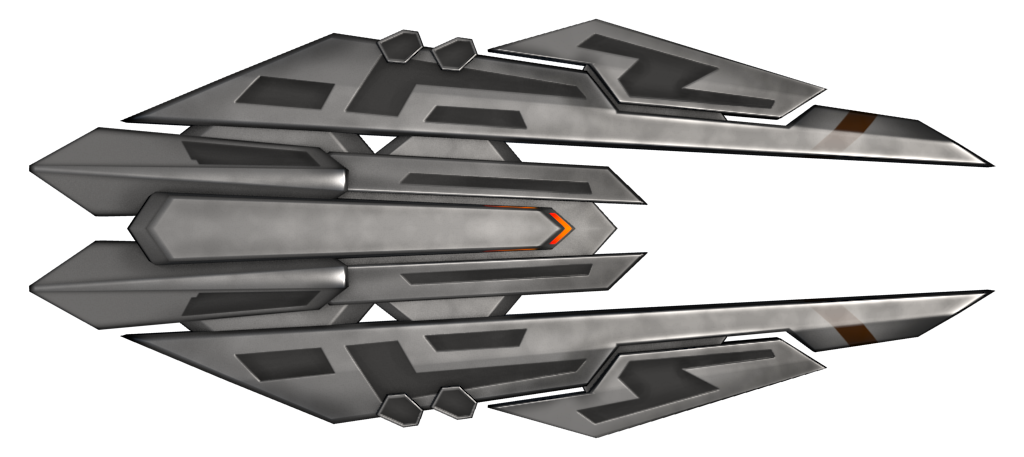
\includegraphics[width=30mm]{./ships/ship14}
\caption{Nave enemiga 17 del planeta 17} \label{figura17}
\end{minipage}

\end{figure}


\begin{figure}

\begin{minipage}[b]{0.5\linewidth}
\centering
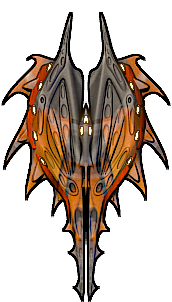
\includegraphics[width=30mm]{./ships/boss3}
\caption{Nave enemiga 18 del planeta 18} \label{figura18}
\end{minipage}
\hspace{0.5cm}
%Planeta final
\begin{minipage}[b]{0.5\linewidth}
\centering
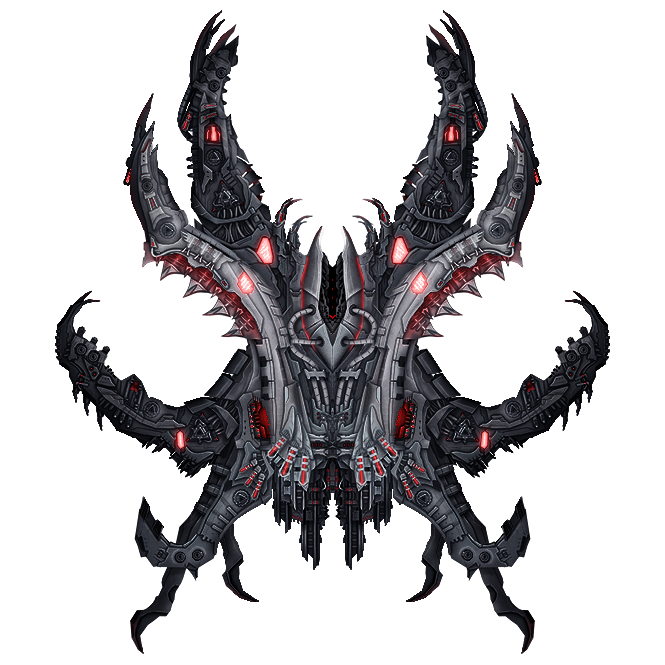
\includegraphics[width=30mm]{./ships/boss4}
\caption{Nave enemiga 19 del planeta 19} \label{figura19}
\end{minipage}

\end{figure}
\cleardoublepage

%player

\cleardoublepage


\end{document}
